% TODO: explain what each variable means
% e.g.: where i_{dq} is the filter output current
\chapter{Mathematical Modeling of VSM}\label{chap:vsm-modeling}

Chapter \ref{chap:vsm-overview} described various VSM topologies available in
the literature. Based on a comparison with SGs, we concluded the CVSM is the  
most suitable for operation in weak grids, since it provides voltage and
frequency support, and has good stability since it is PLL free and has virtual
impedance. 

In this Chapter, we provide a detailed mathematical modeling of the CVSM
topology, with some modifications to include the dynamics of the excitation and
damper windings. In other words, we will aim to model the CVSM as SGs of
different orders, such as the classical, the 1-axis and 2-axis models. First, a
brief overview of the system topology and control scheme is illustrated. Then,
the mathematical modeling of each physical and digital component is presented.
Finally, we calculate the equilibrium point of the entire system for conducting
numerical simulations in the next Chapter.

\section{Overall Sytem Topology and Control Scheme}

This Section presents an overview of the system topology and control scheme, as
depicted in Figure \ref{fig:generic_gfmi}. For simplifying the representation,
just a single phase of the circuit is represented in this image. The DC/AC
inverter is assumed to be a two-level three-phase VSC, with each switch cell is
composed of a fully controllable, unidirectional switch in antiparallel
connection with a diode. A DC source (battery, solar panel or other renewable
resource) and a DC-Link are connected to the DC side of the inverter, whereas a
LCL filter is connected to its AC side before connecting to the bus bar of a AC
power grid. Since this thesis focuses on the control strategy of the grid-side,
the dynamics of the DC source will be ignored, and the DC-link will be considerd
as a ideal constant voltage source.

% TODO: check if this diagram is correct, maybe the signals measured are
% v_dq and i_dq, instead of V_DQ and I_DQ.
\begin{figure}[ht!]
    \centering
    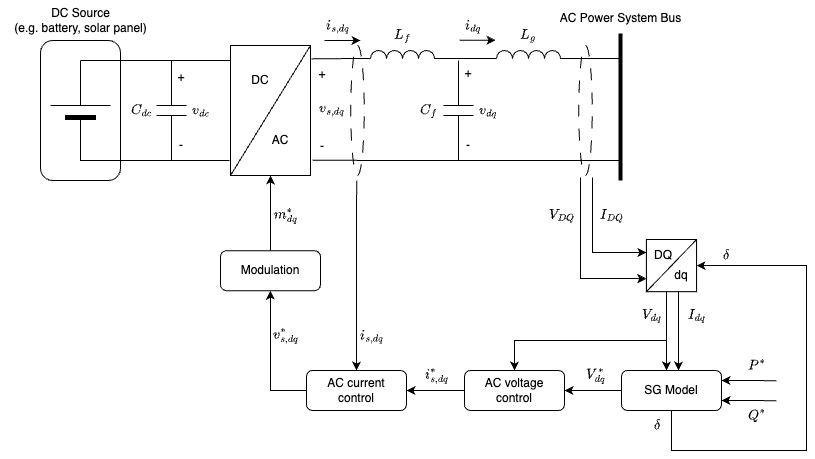
\includegraphics[width=12cm]{images/generic_gfmi.png}
    \caption{Overview of the system topology and control scheme.}
    \label{fig:generic_gfmi}
\end{figure}

As illustrated in Figure \ref{fig:generic_gfmi}, the proposed VSG system is
identical to the CVSM control scheme described in Section \ref{sec:CSVSM},
except for some small modifications. First, the Virtual Inertia and Power
Control, Reactive Power Control and Virtual Impedance blocks of Figure
\ref{fig:CVSM} are grouped in the SG Model block. In other words, we will
represent and implement the active and reactive power regulation in the same 
manner as SGs, including not only the swing equation, but also the excitation
and damping windings dynamics. Moreover, as it will be explained in Section
\ref{sec:modeling_vsm}, the damping power will be calculated based on the
difference between the virtual rotor speed and the synchronous speed
\cite{krause2002analysis,kundur2022power,sauer2017power}. Thus, there is no need
for a PLL.

In addition, since the objective of this thesis is to evaluate the importance of
including the damper winding dynamics, every other damping technique, such as
the Active Damping of the original CVSM in Section \ref{sec:CSVSM}, will not be
implemented. Finally, as it is will be explained in Section
\ref{sec:modeling_vsc}, in multimachine power system simulations, it is common
to express all machines' variables into the Synchronously Rotating Reference
Frame, converting balanced three-phase sinusoidal variations into constants.
Thus, instead of employing $abc-dq0$ transformation, we use here the $DQ-dq$
transformation.

\section{Mathematical Modeling of VSC} \label{sec:modeling_vsc}

In this Section, we describe the assumptions and equations used to model the VSC
illustrated in Figure \ref{fig:generic_gfmi}. The inverter is assumed to be an
ideal two-level three-phase VSC, with each cell being composed of a fully
controllable, unidirectional switch in antiparallel connection with a diode, as
illustrated in Figure \ref{fig:VSC}.

\begin{figure}[ht!]
    \centering
    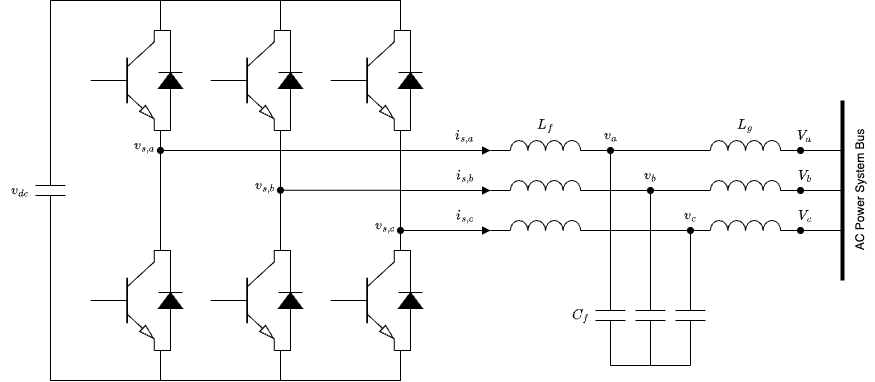
\includegraphics[width=12cm]{images/VSC.png}
    \caption{Overview of the system topology and control scheme.}
    \label{fig:VSC}
\end{figure}

The assumption of an ideal VSC implies in the following \cite{yazdani2010voltage}:
\begin{itemize}
    \item Each transistor or diode acts as a short circuit in its conduction state.
    \item Each transistor or diode switch acts as an open circuit in its blocking state.
    \item The transistors have no turn-off tailing current.
    \item The diodes have no turn-off reverse recovery current.
    \item Transitions from a conduction state to a blocking state, and vice versa, take place instantly.
    \item The AC-side current is a ripple-free DC quantity.
\end{itemize}

Moreover, we employ the averaged-model of the VSC, meaning that the dynamics of
the average values will be analyzed, rather than analyzing the instantaneous
values. By doing so, it is possible to describe the converter dynamics in
function of the modulation signal, which is the main control variable. In the
next subsections, we will present some fundamental theory for developing the
averaged-model of the VSC.

\subsection{PWM Modulation}\label{subsection:pwm}

The two-level three-phase VSC of Figure \ref{fig:VSC} is composed of three
half-bridge converter connected in parallel to a common DC-side voltage source.

\begin{figure}[ht!]
    \centering
    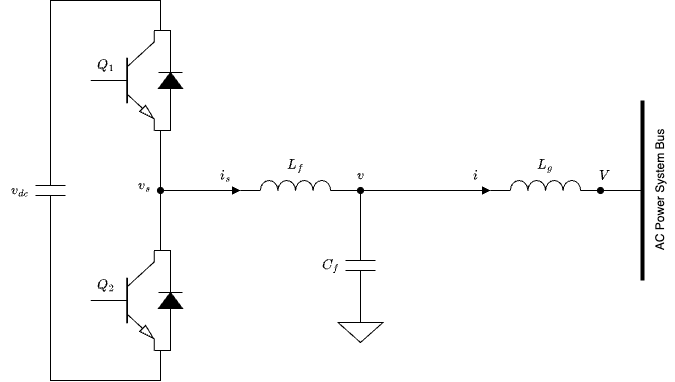
\includegraphics[width=12cm]{images/half_bridge.png}
    \caption{Half-bridge converter.}
    \label{fig:half_bridge}
\end{figure}

The operation of this converter consists in alternating the switches $Q_1$ and
$Q_4$, illustrated in Figure \ref{fig:half_bridge}, which have different
polarities. The turn-on/off commands of these switches can be implemented under
various strategies, but the Pulse-Width Modulation (PWM) is the most popular
technique used in inverters. This technique consists in comparing a periodic
triangular waveform, the carrier signal, with the modulating signal, which is
the desired output signal. The carrier signal has a periodic waveform with
period $T_s$ and varies between -1 and 1, and the switching of $Q_1$ and $Q_4$
is determined by the intersections between the carrier and modulating waveforms
\cite{yazdani2010voltage}.

\newpage
\begin{figure}[ht!]
    \centering
    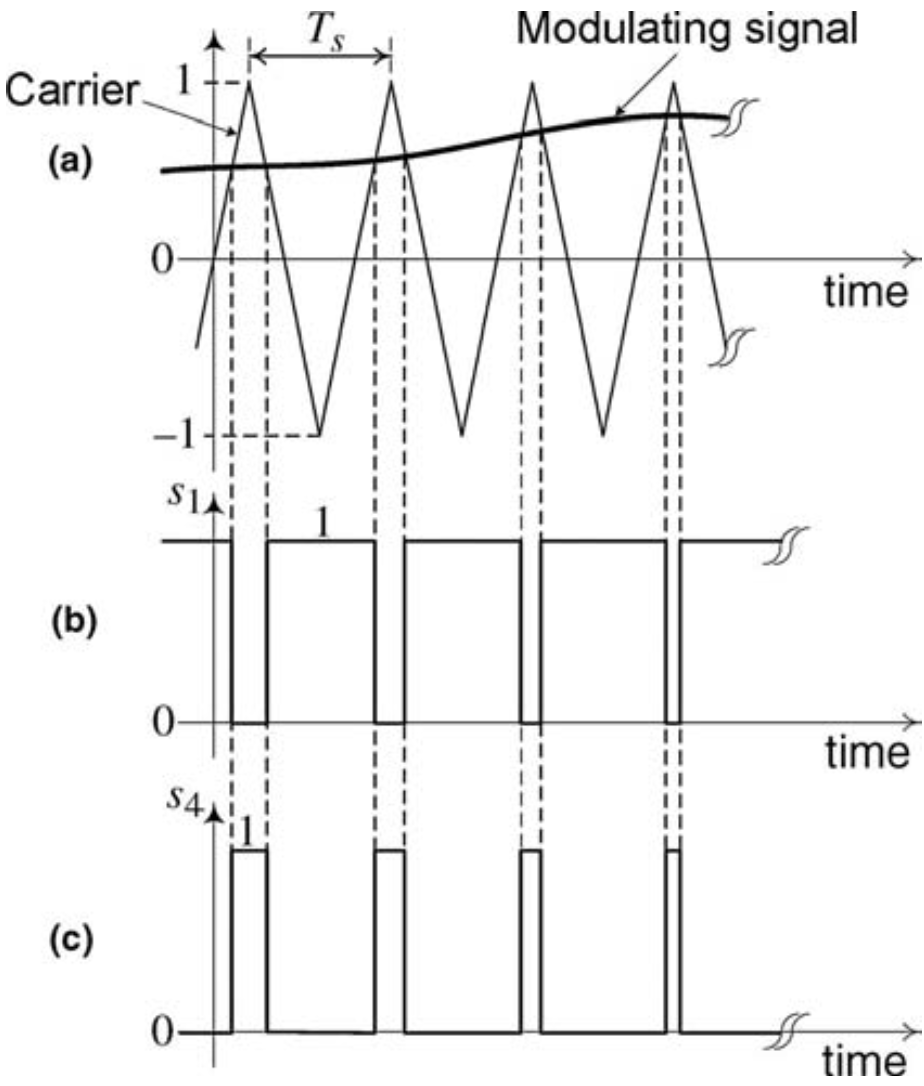
\includegraphics[width=8cm]{images/pwm.png}
    \caption{PWM switching strategy: (a) carrier and modulating waveforms, (b)
    switching function of switch $Q_1$ and (c) switching function of switch
    $Q_4$ \cite{yazdani2010voltage}.}
    \label{fig:pwm}
\end{figure}

From Figure \ref{fig:pwm}, we notice that the half-bridge converter can be
characterized by the following equations when controlled by PWM.

\begin{equation}\label{eq:v_s}
    \begin{aligned}
        &s_1 + s_4 \equiv 1\\
        &v_s = \frac{v_{dc}}{2} s_1(t) - \frac{v_{dc}}{2} s_4(t)
    \end{aligned}
\end{equation}
\noindent where $s_1$ and $s_4$ are the switching signals for $Q_1$ and $Q_4$,
respectively, $v_{dc}$ is the voltage provided by the DC source and $v_s$ is the
voltage in the switching stage of the converter, as illustrated in Figure
\ref{fig:half_bridge}.

\subsection{Park's Transformation (\textit{dq0}-Transformation)}\label{subsection:park}

In power systems, the $dq0$-transformation, also known as Park's transformation,
consists in converting from the static \textit{abc} frame to a rotating $dq0$
frame. The main objective of this transformation is to reduce a three-phase
sinusoidal components into two-dimensional DC components, and therefore it
results in relatively simple dynamic models that can be controlled through
classical PID controllers.

This transformation slightly differs from author to author depending on the
choice of the leading and lagging components. For instance, in
\cite{sauer2017power} the authors consider the a-axis and the q-axis initially
aligned, while in \cite{krause2002analysis} the authors considers the a-axis and
the d-axis initially aligned.

\begin{figure}[!ht]
    \centering
    \begin{subfigure}{.5\textwidth}
      \centering
      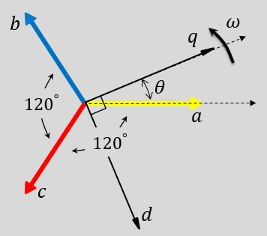
\includegraphics[width=5cm]{images/park_transform_axes_01.png}
      \caption{The a-axis and the q-axis are initially aligned.}
      \label{fig:park_transform_axes_01}
    \end{subfigure}%
    \begin{subfigure}{.5\textwidth}
      \centering
      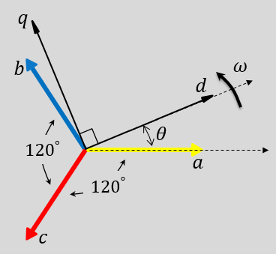
\includegraphics[width=5cm]{images/park_transform_axes_02.png}
      \caption{The a-axis and the d-axis are initially aligned.}
      \label{fig:park_transform_axes_2}
    \end{subfigure}
    \caption{Different representations of \textit{dq0} frame.}
    \label{fig:park_transform_axes}
\end{figure}

In this thesis, the a-axis and the q-axis are chosen to be initially aligned. In this
case, the Park transformation can be expressed by the following transformation matrix
from $abc$ frame to the rotating $dq0$ frame.

\begin{equation}
    T_{dq0} = 
    \frac{2}{3}
    \begin{bmatrix}
        \sin{(\omega t)} & \sin{\left(\omega t - \frac{2\pi}{3}\right)} & \sin{\left(\omega t + \frac{2\pi}{3}\right)}\\
        \cos{(\omega t)} & \cos{\left(\omega t - \frac{2\pi}{3}\right)} & \cos{\left(\omega t + \frac{2\pi}{3}\right)}\\
        \frac{1}{2} & \frac{1}{2} & \frac{1}{2}
    \end{bmatrix}
    \label{eq:park_transformation}
\end{equation}

\noindent where $\omega t$ is the angle of the $q$-axis with respect to the
$a-$axis at time $t$. The inverse transformation can be expressed by the
following matrix.

\begin{equation}
    T_{dq0}^{-1} = 
    \begin{bmatrix}
        \sin{(\omega t)} & \cos{(\omega t)} & 1 \\
        \sin{(\omega t-\frac{2\pi}{3})} & \cos{(\omega t-\frac{2\pi}{3})} & 1 \\
        \sin{(\omega t+\frac{2\pi}{3})} & \cos{(\omega t+\frac{2\pi}{3})} & 1 \\
    \end{bmatrix}
    \label{eq:park_inverse_transformation}
\end{equation}

% TODO: revise this section, it is very bad/fucked up
\subsection{Averaged Model of VSC}

Applying the Kirchhoff's current and voltage laws to the circuit in Figure
\ref{fig:VSC}, the following relationship between voltage and currents can be
obtained.

\begin{equation}
    \begin{cases}
        L_f \frac{di_{s,abc}}{dt} = v_{s,abc} - v_{abc}\\
        C_f \frac{dv_{abc}}{dt} = i_{s,abc} - i_{abc}\\
        L_g \frac{di_{abc}}{dt} = v_{abc} - V_{abc}\\
    \end{cases}
    \label{eq:vsc_abc}
\end{equation}
\noindent where $i_{s,abc} = \begin{bmatrix}i_{s,a} & i_{s,b}
&i_{s,c}\end{bmatrix}^\top$ is the vector of currents at the switching stage of
the converter, $v_{abc} = \begin{bmatrix}v_{a} & v_{b} &
v_{c}\end{bmatrix}^\top$ is the vector of voltages across the filter capacitors,
$i_{abc} = \begin{bmatrix}i_{a} & i_{b} &i_{c}\end{bmatrix}^\top$ is the vector
of output currents of the LCL filter and $V_{abc} = \begin{bmatrix}V_{a} & V_{b}
&V_{c}\end{bmatrix}^\top$ is the vector of output voltages of the LCL filter.
Moreover, $L_f$, $C_f$ and $L_g$ are the filter inductances and capacitance.

From the theory of nonlinear systems, it is possible to average a signal by
applying the following operator \cite{yazdani2010voltage}:

\begin{equation*}
    \bar{x}(t) = \frac{1}{T_s}\int_{t-T_s}^{T_s}x(\tau)d\tau
\end{equation*}

\noindent where $x(t)$ denotes any physical quantity, and the overbar denotes
its average. Thus, by integrating both sides of the first equation in Equation
\ref{eq:vsc_abc} for a single-phase:

\begin{equation*}
    \frac{1}{T_s} \int_0^{T_s}\left(L_f\frac{di_{s}(\tau)}{dt}\right)d\tau = \frac{1}{T_s} \int_0^{T_s} (v_{s}(\tau) - v(\tau))d\tau
\end{equation*}

\begin{equation*}
    L_f \frac{d}{dt}\left(\frac{1}{T_s}\int_0^{T_s}i_{s}(\tau)d\tau\right) = \frac{1}{T_s}\int_0^{T_s}v_{s}(\tau)d\tau - \frac{1}{T_s}\int_0^{T_s}v(\tau)d\tau
\end{equation*}

\begin{equation*}
    L_f \frac{d\bar{i}_{s}}{dt} = \frac{1}{T_s}\int_0^{T_s}v_{s}(\tau)d\tau - \bar{v}
\end{equation*}

From Equation \ref{eq:v_s}:

\begin{equation*}
    L_f \frac{d\bar{i}_{s}}{dt} = \frac{1}{T_s}\int_0^{T_s}\left(\frac{v_{dc}}{2}s_1(\tau) - \frac{v_{dc}}{2}s_4(\tau)\right)d\tau - \bar{v}
\end{equation*}

Moreover, since $s_1 + s_4 \equiv 1$ over the period $T_s$, let $d$ denote the
duty cycle of the inverter, then if $s_1 = 1$ over $dT_s$ seconds, then $s_4 =
1$ must hold for $(T_s - dT_s)$ seconds, as illustrated in Figure \ref{fig:pwm}.
Therefore, the above equation becomes:

\begin{equation*}
    L_f \frac{d\bar{i}_{s}}{dt} = \frac{v_{dc}}{2}(2d - 1) - \bar{v}
\end{equation*}

Or, replacing $m = 2d - 1$, where $m$ is the modulation amplitude, and
considering the three-phases of the system:

\begin{equation*}
    L_f \frac{d\bar{i}_{s,abc}}{dt} = m_{abc}\frac{v_{dc}}{2} - \bar{v}_{abc}
\end{equation*}

\noindent where $m_{abc}$ is a vector of the modulation amplitudes for each
phase.

Repeating the same procedure to the remaining equations of Equation
\ref{eq:vsc_abc}, the averaged model of the VSC can be described by:

\begin{equation}
    \begin{cases}
       L_f \frac{d\bar{i}_{s,abc}}{dt} = m_{abc}\frac{v_{dc}}{2} - \bar{v}_{abc}\\
       C_f \frac{d\bar{v}_{abc}}{dt} = \bar{i}_{s,abc} - \bar{i}_{abc}\\
       L_g \frac{d\bar{i}_{abc}}{dt} = \bar{v}_{abc} - \bar{V}_{abc}\\
    \end{cases}
    \label{eq:vsc_averaged_abc}
\end{equation}

% TODO: provide step-by-step calculation of the Park's transformation
Moreover, multiplying both side of the equations by the transformation matrix
\ref{eq:park_transformation}, we obtain the averaged model in the $dq0$-frame.

\begin{equation}
    \begin{cases}
       L_f \frac{di_{s,dq}}{dt} = -\omega L_f \mathcal{J}_2 i_{s,dq} + m_{dq}\frac{v_{dc}}{2} - v_{dq}\\
       C_f \frac{dv_{dq}}{dt} = -\omega C_f \mathcal{J}_2 v_{dq} + i_{s,dq} - i_{dq}\\
       L_g \frac{di_{dq}}{dt} = -\omega L_g \mathcal{J}_2 i_{dq} + v_{dq} - V_{dq}\\
    \end{cases}
    \label{eq:vsc_averaged_dq}
\end{equation}

\noindent where the $dq$ subscripts indicate vectors of two dimensions, one
corresponding to the $d-$axis component, and the another to the $q-$axis
component. The entire system is considered symmetrical and balanced, thus the
$0$ component is ignored. Moreover, $\mathcal{J}_2 = \begin{bmatrix}0 & -1\\ 1 &
0\end{bmatrix}$ and the overbar indicating average value is removed for
simplifying the notation.

\section{Mathematical Modeling of VSM} \label{sec:modeling_vsm}

The SG Model illustrated in Figure \ref{fig:generic_gfmi} corresponds to the
outer loop of the system, and is responsible for active and reactive power
regulation. In the topologies presented in Chapter \ref{chap:vsm-overview} the
active and reactive power regulation is implemented through the emulation of the
swing equation and a $Q-V$ droop control, respectively.

In this thesis, the SG Model block will be implemented using the equations of SG
models of different orders, namely the 2-axis, 1-axis and classical models. A
similar implementation can be found in \cite{zhang2013improved,ma2017vsg} for
the 2-axis model, and the implementation of the classical model is equivalent to
that of the original CSVM implementation \cite{darco2015vsm}. However, the
implementation of the 1-axis model is not yet reported in the literature.

The SG Model block is composed of three main subsystems, one for emulating the
swing equation, one for emulating the electromagnetic equations, and one
corresponding to an automatic voltage regulator (AVR).

\begin{figure}[ht!]
    \centering
    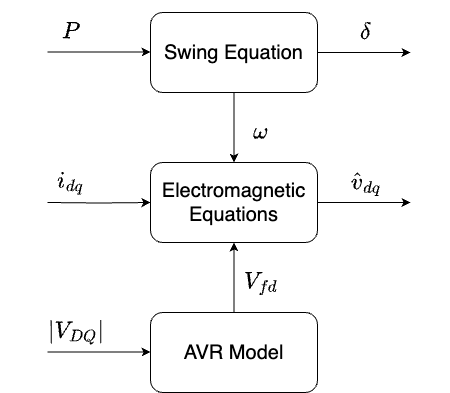
\includegraphics[width=8cm]{images/sm_overall_model.png}
    \caption{Subsystem of the SG Model block.}
    \label{fig:sm_overall_model}
\end{figure}

The digital implementation of the Swing Equation is illustrated by the schema
block in Figure \ref{fig:swing_equation_blocks} where $D$ is the damping
coefficient, $M$ is the inertia coefficient, $\Delta\omega = \omega - \omega_s$
corresponds to the frequency deviation from the synchronous speed, $P^{\star}$
is the active power setpoint, $P$ is the converter output active power and
$\delta$ is the virtual rotor angular position with respect to the synchronously
rotating frame.

\begin{figure}[ht!]
    \centering
    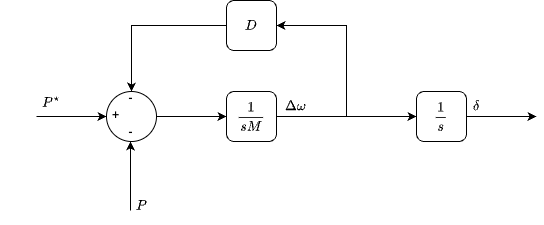
\includegraphics[width=12cm]{images/swing_equation_blocks.png}
    \caption{Schema block of the swing equation.}
    \label{fig:swing_equation_blocks}
\end{figure}

Moreover, the AVR Model is implemented according to Figure \ref{fig:avr_blocks},
where $V^{\star}$ is the output voltage setpoint, provided from the power flow
calculation, $|V_{DQ}|$ is the converter output voltage magnitude, $T_A$ is the
amplifier time constant, $K_A$ is the amplifier gain, $V_R$ is the exciter
input, $T_F$ and $K_F$ are the stabilizing transformer time constant and gain,
respectively, $R_f$ is the rate feedback, $T_E$, $K_E$ and $S_E$ are the exciter
time constant, gain and saturation function, respectively.

\begin{figure}[ht!]
    \centering
    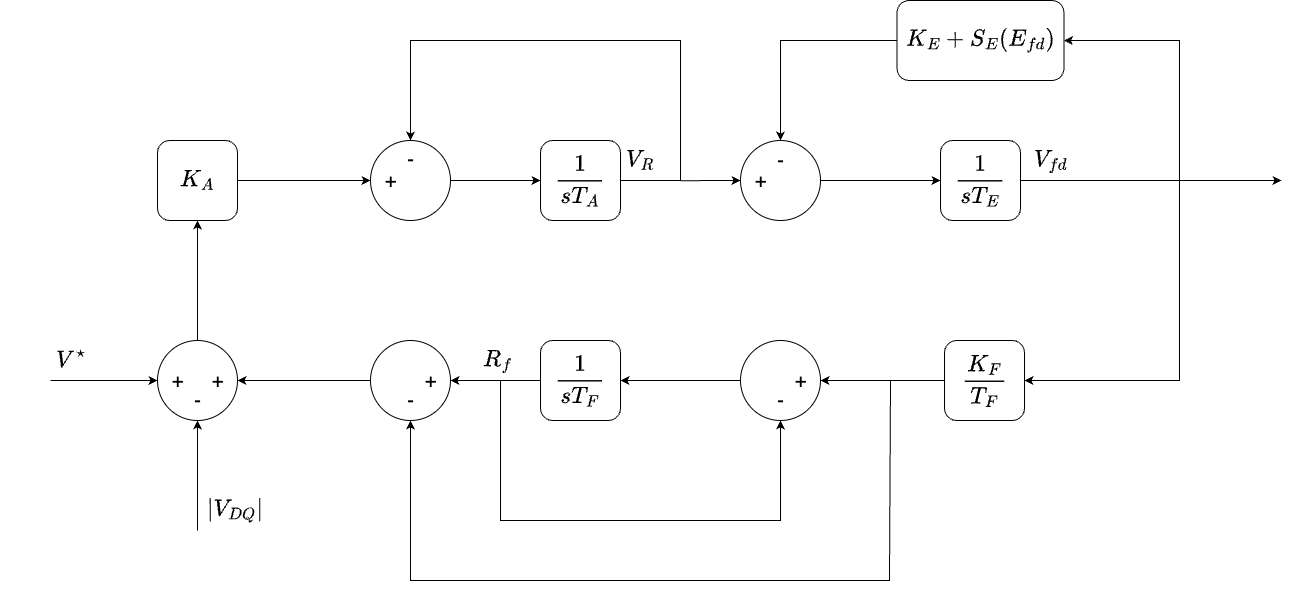
\includegraphics[width=12cm]{images/avr_blocks.png}
    \caption{Schema block of the AVR.}
    \label{fig:avr_blocks}
\end{figure}

The Swing Equation and AVR Model are the same for all SG implementations. It is
important to note that usually the active power setpoint $P^{\star}$ is provided
to the generator by its governor. However, in this thesis $P^{\star}$ will be
considered constant and equal to the active power resulting from the power flow
calculation. This approximation results from the fact that the dynamics of the
governor are normally much slower than that of the exciter
\cite{knazkins2004stability}.

On the other hand, the electromagnetic equations for the 2-axis, 1-axis and
classical model are different, according to the number of damper windings taken
into in consideration. Please refer to \cite{sauer2017power} and to the Appendix
\ref{chap:sg_modeling} for more details about modeling of SGs. The schema blocks
for the electromagnetic equations of each model are illustrated in Figures
\ref{fig:2_axis_block}, \ref{fig:1_axis_block} and \ref{fig:classical_block}.

\begin{figure}[ht!]
    \centering
    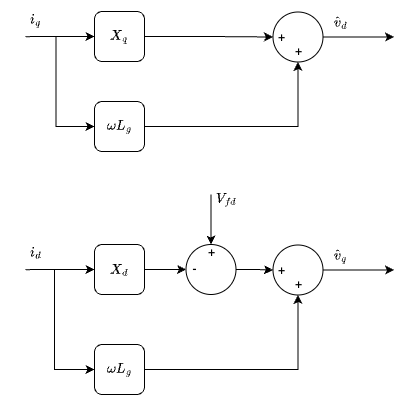
\includegraphics[width=5cm]{images/classical_block.png}
    \caption{Schema block of electromagnetic equations of the classical model.}
    \label{fig:classical_block}
\end{figure}

\newpage
\begin{figure}[ht!]
    \centering
    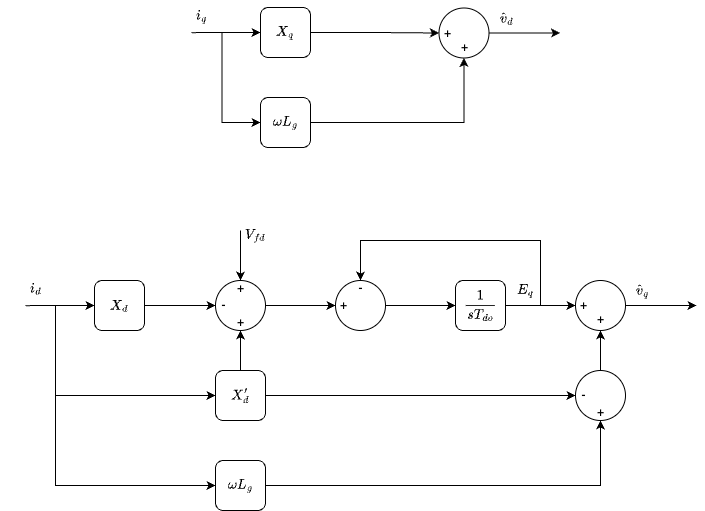
\includegraphics[width=12cm]{images/1_axis_block.png}
    \caption{Schema block of electromagnetic equations of the 1-axis model.}
    \label{fig:1_axis_block}
\end{figure}

\begin{figure}[ht!]
    \centering
    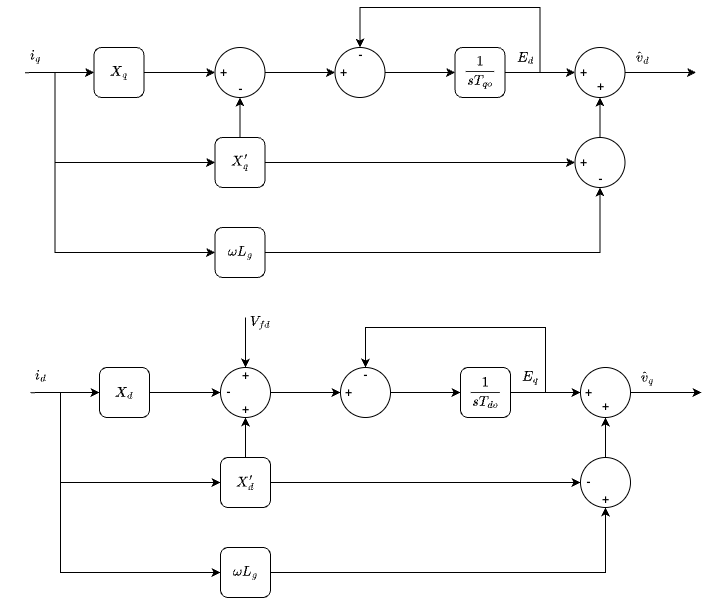
\includegraphics[width=12cm]{images/2_axis_block.png}
    \caption{Schema block of electromagnetic equations of the 2-axis model.}
    \label{fig:2_axis_block}
\end{figure}

In Figures \ref{fig:2_axis_block}, \ref{fig:1_axis_block} and
\ref{fig:classical_block}, $X_d$ and $X_q$ are the transient reactances, $X_d'$
and $X_d'$ are the subtransient reactances, $T_{do}$ and $T_{qo}$ are the
windings time constants, $E_d$ and $E_q$ are the transient voltages and $L_g$ is
the converter LCL filter outer inductance. The feedforward terms $\omega L_gi_d$
and $\omega L_gi_d$ are added to compensate the converter LCL filter outer
inductance such that the filter output voltage behaves similarly to a SG
terminal voltage. The dynamic equations describing the SG Model block are:

\begin{equation*}
    \begin{aligned}
        &\textbf{2-axis SG}\\
        &\begin{cases}
            \frac{d\delta}{dt} &= \omega_s \Delta\omega\\
            M\frac{\Delta\omega}{dt} &= -D\Delta\omega + P^{\star} - P\\
            T_{do}' \frac{E_q}{dt} &= -E_q - (X_d - X_d')I_d + V_{fd}\\
            T_{qo}' \frac{E_d}{dt} &= -E_d + (X_q - X_q')I_q\\
            T_E \frac{dV_{fd}}{dt} &= -\left(K_E + S_E(V_{fd})\right)V_{fd} + V_R \\
            T_F \frac{dR_f}{dt} &= -R_f + \frac{K_F}{T_F}V_{fd} \\
            T_A \frac{dV_R}{dt} &= -V_R + K_A R_f - \frac{K_A K_F}{T_F}V_{fd} + K_A (V^{\star} - |V_{DQ}|)
        \end{cases}
    \end{aligned}
\end{equation*}

\begin{equation*}
    \begin{aligned}
        &\textbf{1-axis SG}\\
        &\begin{cases}
            \frac{d\delta}{dt} &= \omega_s \Delta\omega\\
            M\frac{\Delta\omega}{dt} &= -D\Delta\omega + P^{\star} - P\\
            T_{do}' \frac{E_q}{dt} &= -E_q - (X_d - X_d')I_d + V_{fd}\\
            T_E \frac{dV_{fd}}{dt} &= -\left(K_E + S_E(V_{fd})\right)V_{fd} + V_R \\
            T_F \frac{dR_f}{dt} &= -R_f + \frac{K_F}{T_F}V_{fd} \\
            T_A \frac{dV_R}{dt} &= -V_R + K_A R_f - \frac{K_A K_F}{T_F}V_{fd} + K_A (V^{\star} - |V_{DQ}|)
        \end{cases}
    \end{aligned}
\end{equation*}

\begin{equation*}
    \begin{aligned}
        &\textbf{Classical SG}\\
        &\begin{cases}
            \frac{d\delta}{dt} &= \omega_s \Delta\omega\\
            M\frac{\Delta\omega}{dt} &= -D\Delta\omega + P^{\star} - P\\
            T_E \frac{dV_{fd}}{dt} &= -\left(K_E + S_E(V_{fd})\right)V_{fd} + V_R \\
            T_F \frac{dR_f}{dt} &= -R_f + \frac{K_F}{T_F}V_{fd} \\
            T_A \frac{dV_R}{dt} &= -V_R + K_A R_f - \frac{K_A K_F}{T_F}V_{fd} + K_A (V^{\star} - |V_{DQ}|)
        \end{cases}
    \end{aligned}
\end{equation*}

\section{Mathematical Modeling of Cascaded PI Controller}

As described in Chapter \ref{chap:vsm-overview}, the original implementations of
the main VSM topologies did not considered cascaded loops. Instead, they simply
generated the reference current and voltage for controlling the converter via
$P-\omega$ (realized as the SG swing equation) and $Q-V$ droop laws.

However, in addition to the active and reactive power control, modifications in
the original topologies described in Chapter \ref{chap:vsm-overview} considered
an additional cascaded inner loop to realize the zero-error tracking of the
converter output current or voltage reference, thus ensuring accurate execution
of the outer loop control, which regulates the active and reactive powers
\cite{blaabjerg2018control}. In the CVSM topology, a double-loop PI voltage and
current control is used to further improve the control dynamics, and better
dampen the resonances caused by the converter output filters
\cite{darco2015vsm}.

In Figure \ref{fig:cascaded_pi}, we simplify the block diagram of Figure
\ref{fig:CVSM_cascaded}, assuming that the feed-forward terms are always
included ($k_{ffi} = k_{ffv} = 1$) and removing the active damping terms.
Moreover, we change the variable names to those to be used in this thesis.

\begin{figure}[ht!]
    \centering
    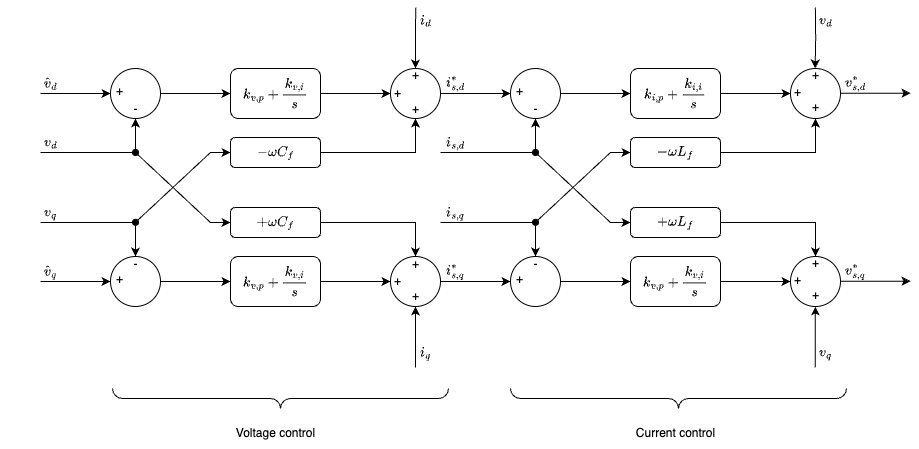
\includegraphics[width=12cm]{images/cascaded_pi.png}
    \caption{Block diagram of the cascaded PI controller.}
    \label{fig:cascaded_pi}
\end{figure}

It is important to note that the feed-forward terms are used for decoupling the
dynamics of the converter and the AC power grid, improving the disturbance
rejection capability and avoiding the converter's start up transients
\cite{yazdani2010voltage}. The block diagram of Figure \ref{fig:cascaded_pi} can
be mathematically described by \cite{darco2015vsm,tayyebi2020power}:

\begin{equation}
    \begin{cases}
        \dot{x}_{v,dq} = \hat{v}_{dq} - v_{dq}\\
        i_{s,dq}^{\star} = i_{dq} + \omega C_f \mathcal{J}_2 v_{dq} + k_{v,p}\mathcal{I}_2 (\hat{v}_{dq} - v_{dq}) + k_{v,i}\mathcal{I}_2 x_{v,dq} 
    \end{cases}
    \label{eq:voltage_control}
\end{equation}

\begin{equation}
    \begin{cases}
        \dot{x}_{i,dq} = i_{s,dq}^{\star} - i_{s,dq}\\
        v_{s,dq}^{\star} = v_{dq} + \omega L_f \mathcal{J}_2 i_{s,dq} + k_{i,p}\mathcal{I}_2 (i_{s,dq}^{\star} - i_{s,dq}) + k_{i,i}\mathcal{I}_2 x_{i,dq} 
    \end{cases}
    \label{eq:current_control}
\end{equation}

\noindent where $\mathcal{I}_2$ is the identity matrix of order 2 and $x_{v,dq}$
and $x_{i,dq}$ are the integrators' internal state. The reference voltage
$v_{s,dq}^{\star}$ is then used for generating the modulation signal for
controlling the converter such that $v_{s,dq} = v_{s,dq}^{\star}$.

\section{Calculation of Equilibrium Point}


\begin{equation}
    \begin{cases}
        L_f \frac{di_{s,dq}}{dt} &= -\omega L_f \mathcal{J}_2 i_{s,dq} + m_{dq}\frac{v_{dc}}{2} - v_{dq}\\
        C_f \frac{dv_{dq}}{dt} &= -\omega C_f \mathcal{J}_2 v_{dq} + i_{s,dq} - i_{dq}\\
        L_g \frac{di_{dq}}{dt} &= -\omega L_g \mathcal{J}_2 i_{dq} + v_{dq} - V_{dq}\\
        \frac{d\delta}{dt} &= \omega_s \Delta\omega\\
        M\frac{\Delta\omega}{dt} &= -D\Delta\omega + P^{\star} - P\\
        T_{do}' \frac{E_q}{dt} &= -E_q - (X_d - X_d')I_d + V_{fd}\\
        T_{qo}' \frac{E_d}{dt} &= -E_d + (X_q - X_q')I_q\\
        T_E \frac{dV_{fd}}{dt} &= -\left(K_E + S_E(V_{fd})\right)V_{fd} + V_R \\
        T_F \frac{dR_f}{dt} &= -R_f + \frac{K_F}{T_F}V_{fd} \\
        T_A \frac{dV_R}{dt} &= -V_R + K_A R_f - \frac{K_A K_F}{T_F}V_{fd} + K_A (V^{\star} - |V_{DQ}|)\\
        \dot{x}_{v,dq} &= \hat{v}_{dq} - v_{dq}\\
        \dot{x}_{i,dq} &= i_{s,dq}^{\star} - i_{s,dq}\\
    \end{cases}
    \label{eq:complete_model}
\end{equation}

\begin{equation}
    \begin{cases}
        L_f \frac{di_{s,dq}}{dt} &= -\omega L_f \mathcal{J}_2 i_{s,dq} + m_{dq}\frac{v_{dc}}{2} - v_{dq}\\
        C_f \frac{dv_{dq}}{dt} &= -\omega C_f \mathcal{J}_2 v_{dq} + i_{s,dq} - i_{dq}\\
        L_g \frac{di_{dq}}{dt} &= -\omega L_g \mathcal{J}_2 i_{dq} + v_{dq} - V_{dq}\\
        \frac{d\delta}{dt} &= \omega_s \Delta\omega\\
        M\frac{\Delta\omega}{dt} &= -D\Delta\omega + P^{\star} - P\\
        T_{do}' \frac{E_q}{dt} &= -E_q - (X_d - X_d')I_d + V_{fd}\\
        T_{qo}' \frac{E_d}{dt} &= -E_d + (X_q - X_q')I_q\\
        T_E \frac{dV_{fd}}{dt} &= -\left(K_E + S_E(V_{fd})\right)V_{fd} + V_R \\
        T_F \frac{dR_f}{dt} &= -R_f + \frac{K_F}{T_F}V_{fd} \\
        T_A \frac{dV_R}{dt} &= -V_R + K_A R_f - \frac{K_A K_F}{T_F}V_{fd} + K_A (V^{\star} - |V_{DQ}|)\\
        \dot{x}_{v,dq} &= \hat{v}_{dq} - v_{dq}\\
        \dot{x}_{i,dq} &= i_{s,dq}^{\star} - i_{s,dq}\\
    \end{cases}
    \label{eq:complete_model}
\end{equation}

% Draw diagram with converter and control blocks
% Justify why a two level converter is used
% Justify why average model is used
% Justify PWM modulation
% Highlight differences from the original CVSM